%!TEX root = ../main.tex

\section*{Results}

  We have developed \hl{insert package name here}, a flexible and modular pipeline for 16S data analysis.
  It incorporates various popular, publicly available tools as well as custom Python modules and scripts to facilitate 16S data processing.
  The pipeline workflow is as shown in Figure \ref{fig:mind_pipeline}, it supports the conversion of raw 16S sequence data or counts matrices into co-occurrence networks through multiple methods.
  Each process in the pipeline supports alternate tools for performing the same task, users can use the configuration file to change these values.
  The set of default options for the pipeline can be found in Table \ref{table:default_options}.
  We also provide the users with a set of guidelines to facilitate tool selection as appropriate for their data.

  \begin{table}[h]
    \centering
    \small
    \begin{tabular}{|c|c|c|}
      %\begin{tabularx}{\textwidth}{XXXX}
      \hline
      \textbf{Process} & \textbf{Tool} & \textbf{Parameters} \\
      \hline
      Denoising and Clustering & Deblur & ?? \\
      Taxonomy Assignment & \ac{ncbi} + Blast & ?? \\
      OTU Processing & Dynamic cutoff & ?? \\
      Network Inference & User choice & ?? \\
      \hline
    \end{tabular}
    %\end{tabularx}
    \caption{Default tools and parameters for the pipeline}
    \label{table:default_options}
  \end{table}

  \begin{figure}[h]
    \centering
    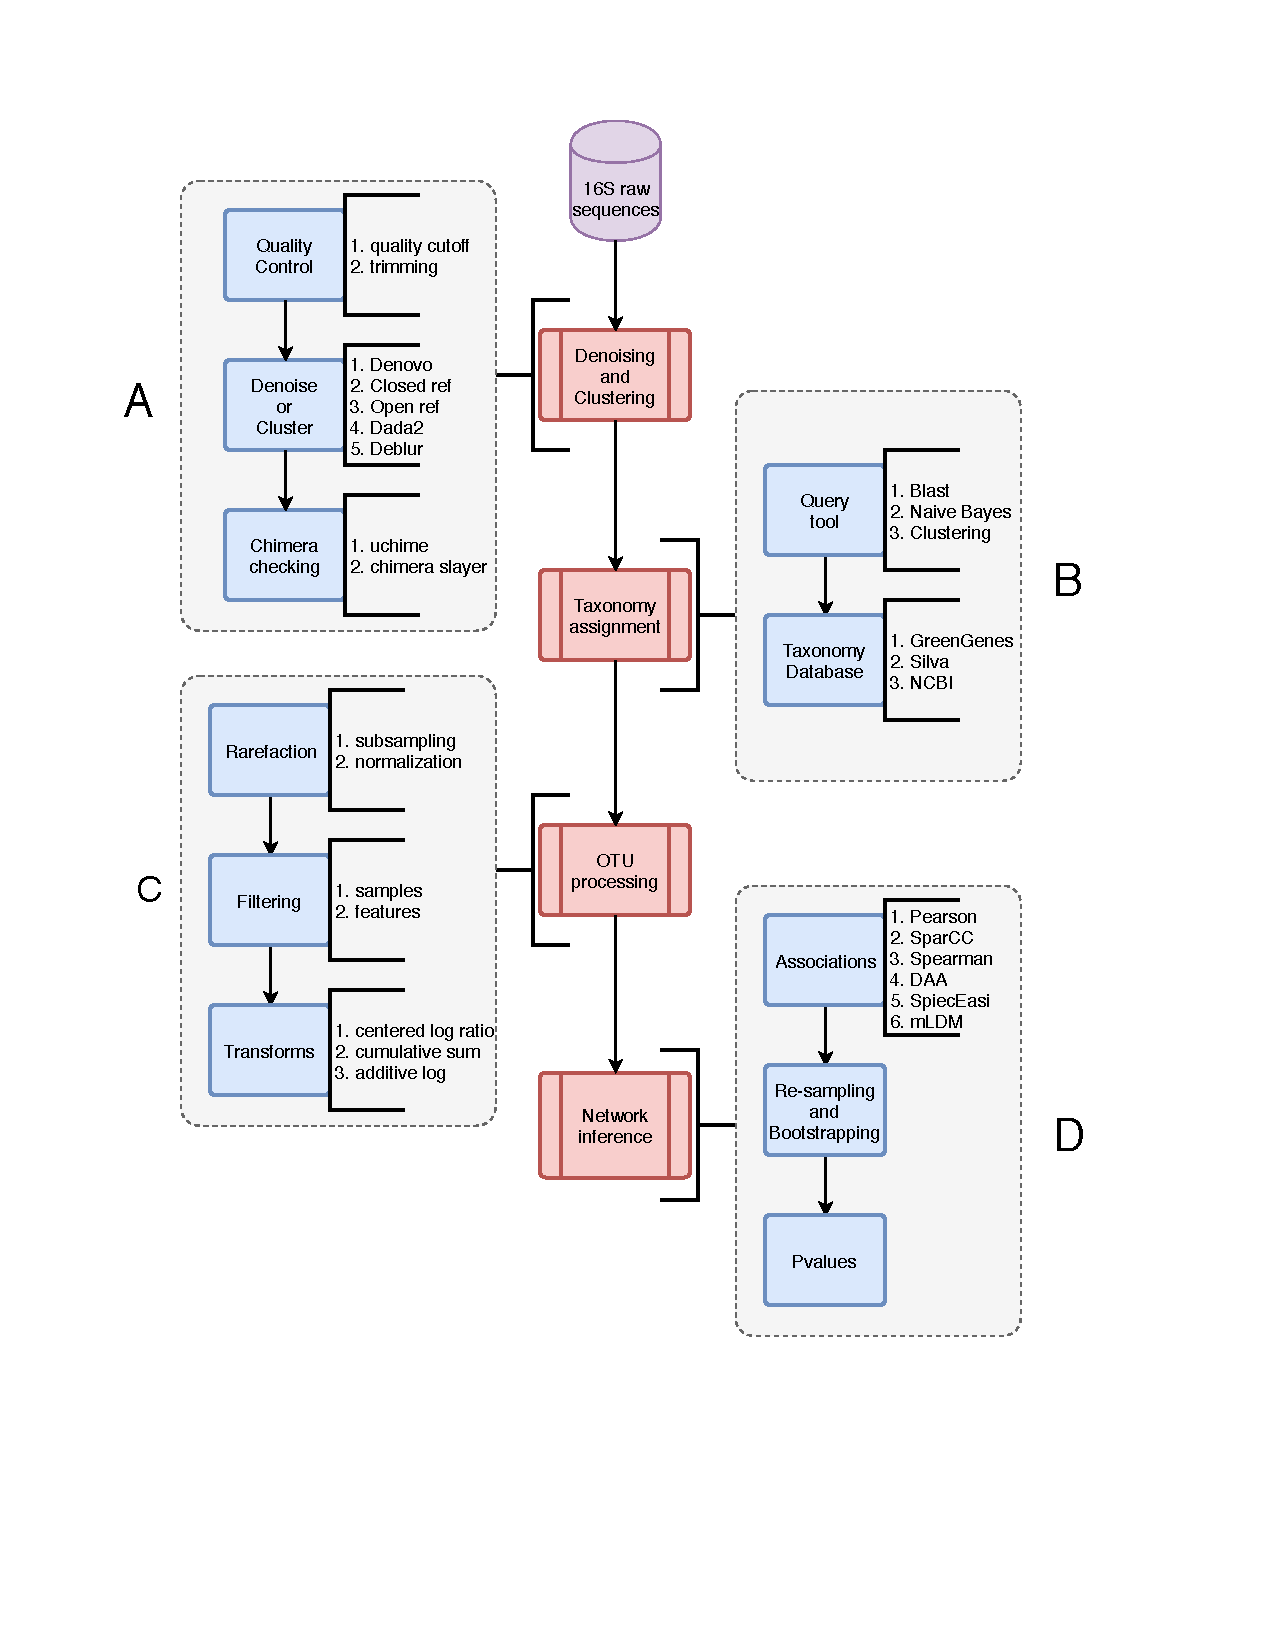
\includegraphics[width=0.9\textwidth]{mind_pipeline.pdf}
    \caption{
      \textbf{The workflow of the microbial co-occurrence analysis pipeline}.
      The processes can be grouped into four major steps: \textbf{(A)} denoising and clustering, \textbf{(B)} taxonomy assignment, \textbf{(C)} \ac{otu}/\ac{esv} processing, and \textbf{(D)} network inference.
      Each step incorporates several processes, each of which in turn have several alternate algorithms for the same task (indicated by the text to the right of the blue boxes).
    }%
    \label{fig:mind_pipeline}
  \end{figure}

  \FloatBarrier

  \subsection*{Variance among co-occurrence networks}

  In order to analyze the effect of different statistical methods on the inferred co-occurrence networks, we generate networks using all possible combinations of methods and estimate the variability in the networks.
  Figure \ref{fig:variance} shows the fraction of total variation among the co-occurrence networks as contributed by each of the four main steps of the pipeline.
  \todo[size=\footnotesize]{Results soon!}

  \begin{figure}[h]
    \centering
    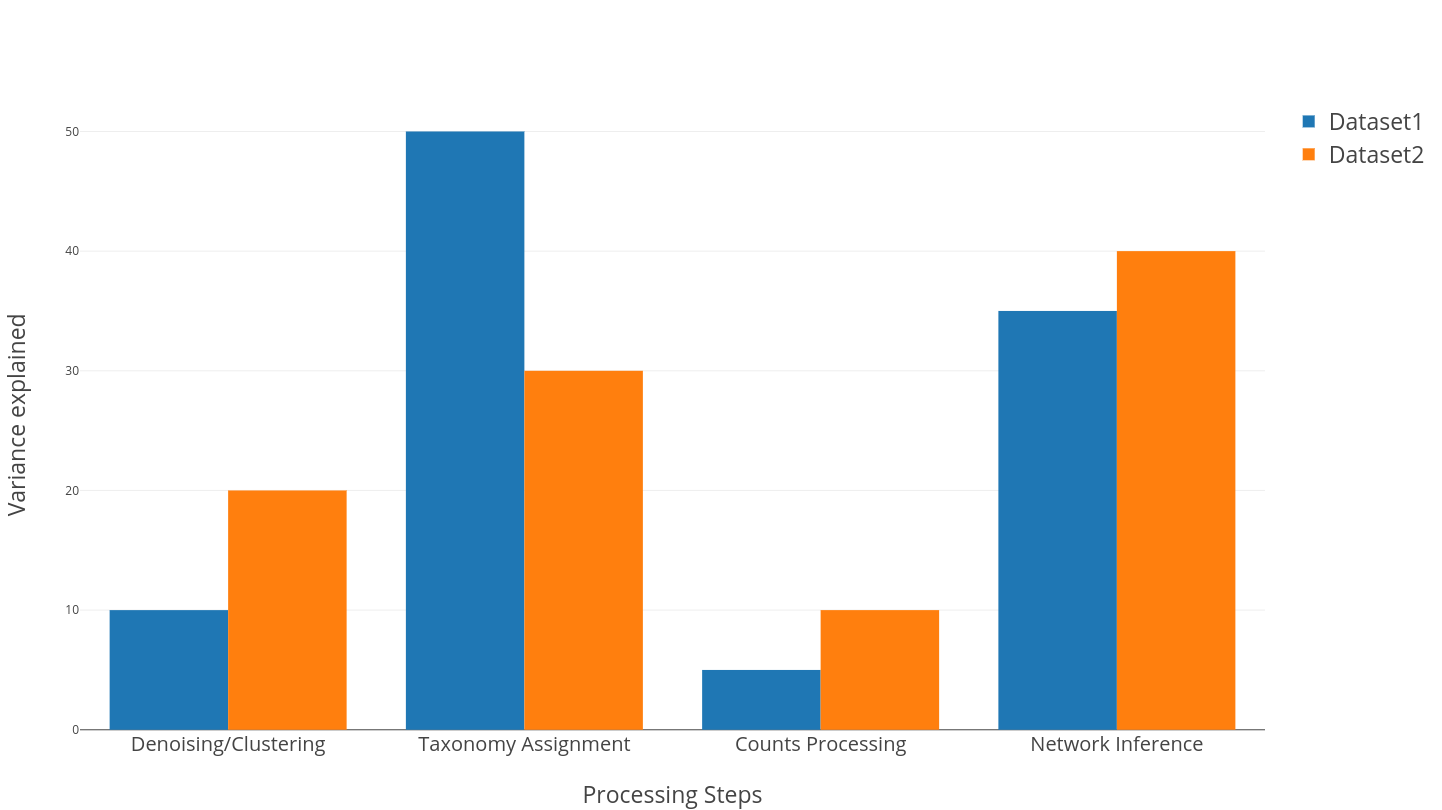
\includegraphics[width=0.9\textwidth]{main_figure.png}
    \caption{\textbf{Percentage of variance in the final co-occurrence network due to each processing step.}}%
    \label{fig:variance}
  \end{figure}


  \FloatBarrier

  \subsection*{Denoising and clustering methods are very dissimilar}

  There is significant variation both in the \ac{otu}/\ac{esv} tables when different combinations of methods are used to generate them.
  We process the same 16S dataset using 5 different methods - open-reference clustering, closed-reference clustering and denovo clustering from \ac{qiime1}~\cite{Caporaso2010}, \ac{dada2}~\cite{Callahan2016} and Deblur~\cite{Amir2017}.
  For each of these methods we use the same taxonomy database (\ac{gg}) to assign taxonomies to the representative sequences.
  We then correlate the abundances of matching taxonomies between every combination of a pair of methods (Figure \ref{fig:all_denoise_reg}).
  The \ac{esv} tables generated by methods that perform denoising are very similar to each other $\sim0.9$ and the \ac{otu} tables generated by the clustering methods are very similar to each other $\sim0.9$, but results of denoising and clustering are highly uncorrelated with each other $\sim0.4$ (Figure \ref{fig:otu_correlations}).

  The common core network (network made up of edges that are predicted by all methods) is very small compared to the total number of edges predicted by all the methods (Figure \ref{fig:denoise_network}).
  In these results, only the denoising method was changed (database used: \ac{gg} and network inference: \ac{sparcc}).

  These comparisons only elucidate the pairwise similarity or dissimilarity of a pair of methods. In order to determine the best method we use synthetically generated reads from an Illumina read simulator called Grinder~\cite{Angly2012}.
  The reads were simulated using the taxonomy distribution profile generated by \ac{qiime1} open-reference clustering using the \hl{FMT} dataset.
  Reference sequences were obtained from \ac{gg} and other metrics such as sampling depths, chimera percentage were estimated from the original sequences.
  Detailed information on all the other settings are provided in the methods section.
  We find that the \ac{qiime1} methods (clustering) are not as robust when compared to the denoising methods in re-generating the same abundance distribution. \todo[size=\footnotesize]{Not yet confirmed}

  \begin{figure}[h]
    \centering
    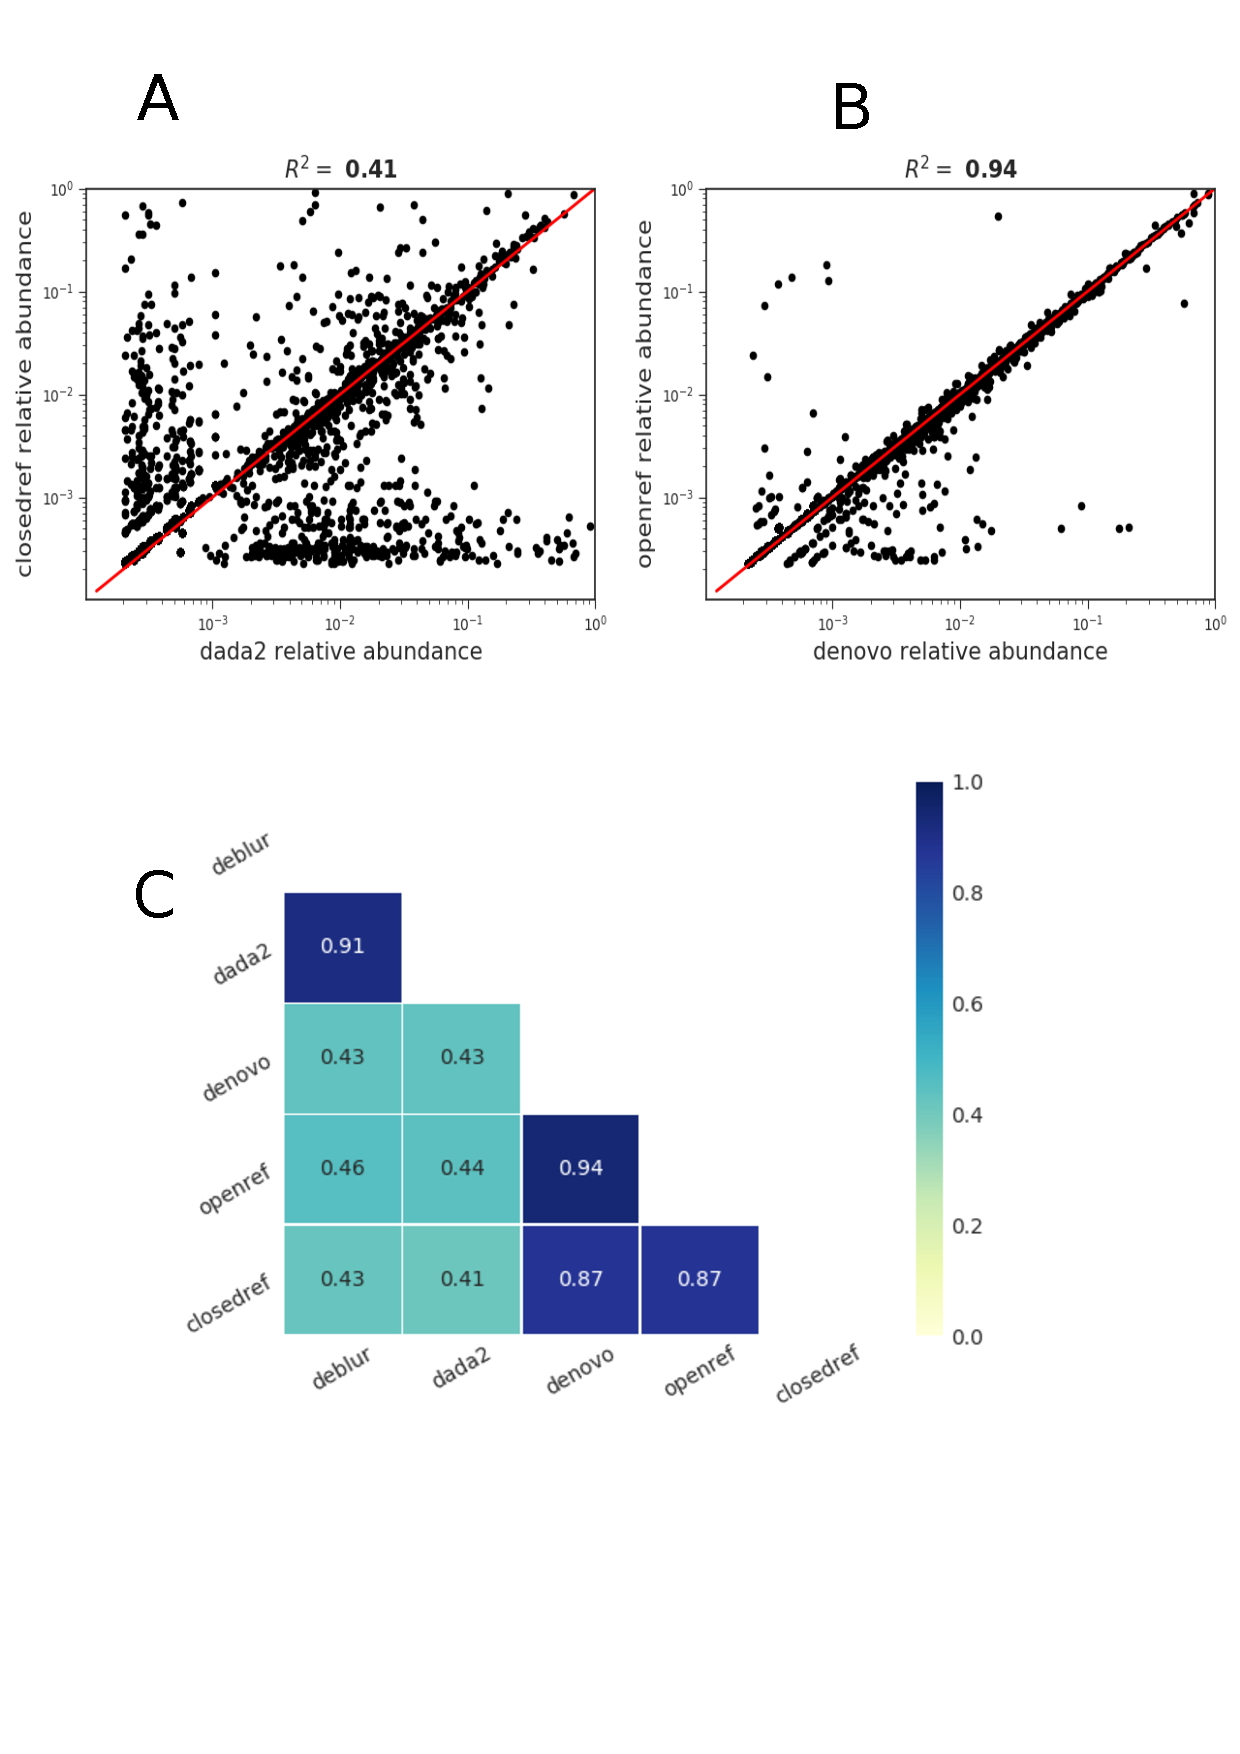
\includegraphics[width=0.9\textwidth]{edited/otu_corr_full.pdf}
    \caption{
      \textbf{Comparison of various denoising and clustering algorithms used in the pipeline}.
      (A, B) Correlation of the abundances of the taxa that are common between the count matrices created by two different methods.
      (A) The best correlation (most similar methods) is between open-reference and denovo.
      (B) The worst correlation (least similar methods) is between open-reference and dada2.
      (C) A heatmap showing the $\mathrm{R}^2$ of all pairwise comparisons of the methods.
    }
    \label{fig:otu_correlations}
  \end{figure}

  \FloatBarrier

  \subsection*{Taxonomy databases vary widely in taxonomy hierarchy and update frequency}

  SILVA and \ac{gg} are two popular 16S databases used for taxonomy identification.
  The two databases vastly differ in terms of their last update status - \ac{gg} was last updated on May 2013 and SILVA was last updated on December 2017 at the time of writing.
  Since updates to taxonomic classifications are frequent, these two databases vary significantly in terms of taxonomy hierarchies~\cite{Balvociute2017}.

  The deblur denoising pipeline was first used to obtain \ac{esv} counts table by processing the FMT 16S sequence data.
  These \ac{esv}s are then assigned a particular taxonomic label using two different reference 16S taxonomy databases - SILVA and \ac{gg}.
  Figure~\ref{fig:tax_comparison} shows that the top 20 most abundant genera in the two resulting taxonomy composition tables are \hl{different}.
  The most abundant genus in the \ac{gg} taxonomy table was \textit{Escherichia} whereas in the SILVA taxonomy table it was \textit{Escherichia-Shigella}.
  These might seem like minor differences, but when comparing a large number of composition tables these problems are hard to diagnose.
  Figure~\ref{fig:tax_comparison_all} shows that the result is very similar when you look at all genera instead of just the top 20 most abundant genera.
  The percentage of this misclassification was found to change with the taxonomy resolution needed.
  The mismatches were $\sim10\%$ at the Phylum level but were seen to go up to $\sim60\%$ at the Species level, as shown in Figure~\ref{fig:tax_mismatches}.
  Moreover, Figure~\ref{fig:venn_tax} shows that there does not seem to exist a correlation between abundance and mismatch.
  This implies that the most abundant sequences are not necessarily the ones that are consistently matched to the same taxonomies in the different reference databases.
  \todo[size=\footnotesize]{Incorporate NCBI}

  These results prompted us to turn to \ac{ncbi} for taxonomy referencing.
  Our reasons for choosing \ac{ncbi} are that it is regularly maintained and updated and accuracy of the assignment is comparable to the SILVA and \ac{gg} reference databases.
  \hl{If we use NCBI we need to show how accurate that is. We can show this using the synthetic data or mock communities}

  \begin{figure}[h]
    \centering
    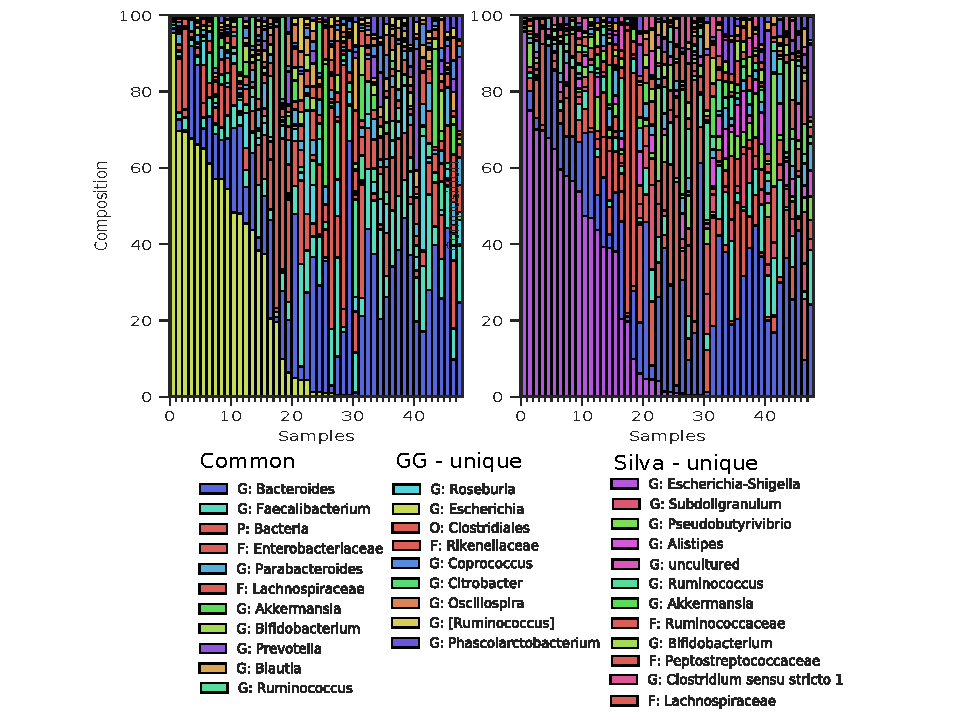
\includegraphics[width=0.9\textwidth]{tax_comp_full.pdf}
    \caption{\textbf{Taxonomy composition of the 20 most abundant genera predicted using different taxonomy references databases}}
    \label{fig:tax_comparison}
  \end{figure}

  \begin{figure}[h]
    \centering
    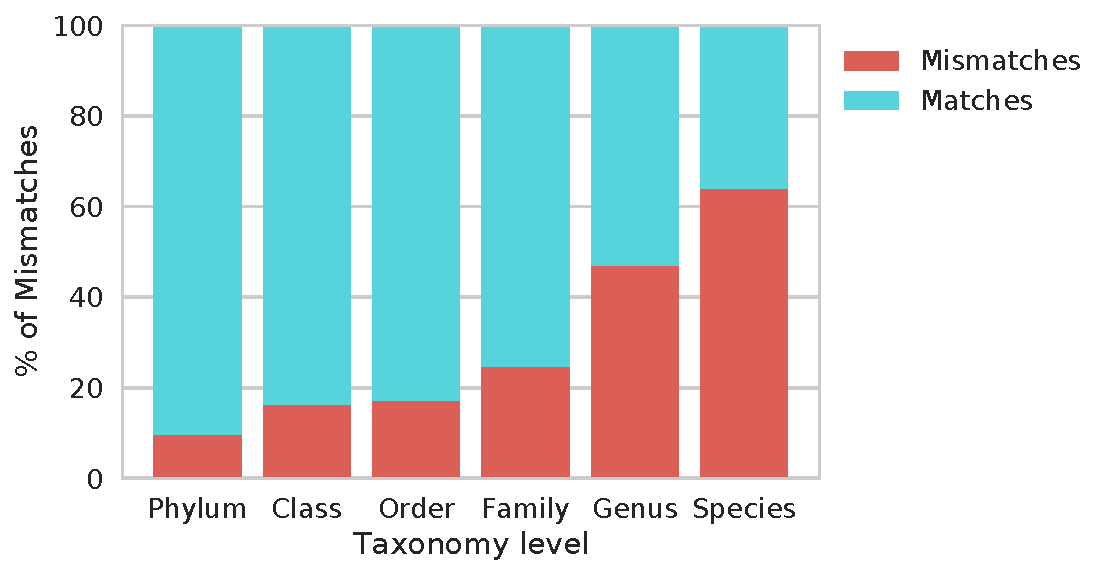
\includegraphics[width=0.95\textwidth]{tax_distance_deblur.pdf}
    \caption{\textbf{Average percentage of mismatches in taxonomy assignment at various taxonomy levels.}}
    \label{fig:tax_mismatches}
  \end{figure}

  \FloatBarrier

  \subsection*{Network inference contributes to the most variance}

  \hl{How did we get these results? What do the figures tell us? What is the conclusion?}

  The taxonomy composition table obtained using the \ac{gg} reference database is used to infer co-occurrence associations between the microbes.

  Different network inference methods infer significantly different association networks.
  We can divide the network inference methods into two sets, the first set of methods (Pearson, Spearman, \ac{sparcc}) infer pairwise correlations while the second set infer direct associations (\ac{spieceasi}, \ac{mldm}, \ac{daa}).
  Our preliminary analysis (Figure \ref{fig:network_comparison}) shows that networks generated using 4 different methods (Pearson, Spearman, \ac{sparcc}, \ac{spieceasi}) are vastly different and the degree of similarity (number of edges that overlapped) between the methods was dependent on the data-set used.
  The abundance profiles of the different data-sets used are show in Figure \ref{fig:abundance_profile}.

  \begin{figure}[h]
    \centering
    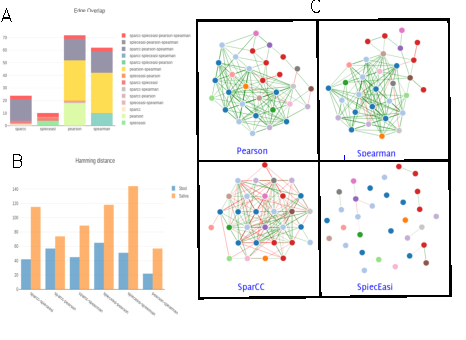
\includegraphics[width=0.9\textwidth]{net_inference_comparison.pdf}
    \caption{
      \textbf{Networks generated using different network inference methods}.
      The four different networks generated by different network inference methods are very dissimilar (C).
      (A) The overlaps between the edges among the network5 generated is shown. The number of edges that are common to all networks are very low (5).
      (B) The hamming distance between the networks is shown. The similarity between various methods was found to vary with the data-source used.
    }
    \label{fig:network_comparison}
  \end{figure}

  \begin{figure}[h]
    \centering
    %\includegraphics[width=17.8cm]{../figures/network_comparison.pdf}
    \caption{\textbf{Core network captures known interactions in vaginal microbiota.} \textbf{(A)} Core network, obtained by taking the intersection between all the different pipelines. \textbf{(B)} Vaginal microbiota network as determined by XXX.}
    \label{fig:real_network}
  \end{figure}

  % TODO: Based on these results: What is the best pipeline we recommend?
  The pipeline and the data visualization tool help the user explore the effect of the various methods on their data.
  Exploring these differences are difficult and inconvenient without the tool since different tools differ in their input and output formats and require inter-converting between the various formats.
  In the case of our pipeline, this is handled automatically.
